\documentclass[11pt,a4paper]{exam}
\usepackage{listings}% C++ & Java
\usepackage{xcolor} % for setting colors
\usepackage{amsmath,amsthm,amsfonts,amssymb,dsfont,mathrsfs}
\usepackage{mathtools}
\usepackage{mathdesign}
\usepackage{textcomp}
\usepackage{ifthen}
\usepackage{tikz}
\usepackage{tkz-graph}
\usepackage{trees}
\usepackage[top=3cm,right=1.5cm,bottom=3cm,left=1.5cm]{geometry} 
%%%%%%%%%%Matrix Package
\usepackage{nicematrix}
 %%%%%%%%%%%%%                                                                                       TablePackage
\usepackage{tabularx}
\usepackage{multirow}
\usepackage{hhline}
%%%%%%%%%%%%%%%%%
\usepackage{hyperref}
\usepackage{color,graphicx}
\usepackage[Kashida]{xepersian}
%%%%%%%%%%%%%%%
%پکیج الگوریتم 
\usepackage{algpseudocode}
\usepackage{algorithmicx}
%%%%%%
\usetikzlibrary {shapes.geometric}

%%%%%%%
\algrenewcommand\algorithmicwhile{\textbf{am\’\i g}}
\algrenewcommand\algorithmicdo{\textbf{v\’egezd el}}
\algrenewcommand\algorithmicwhile{\textbf{am\’\i g}}
\algrenewcommand\algorithmicdo{\textbf{v\’egezd el}}
\algrenewtext{EndWhile}{\algorithmicwhile\ \algorithmicend}
\algnewcommand\algorithmicto{\textbf{to}}
\algsetblock[<block>]{<start>}{<end>}
{<lifetime>}{<indent>}
\algnotext[<block>]{<ending command>}
%%%%%%%%%% C++ & Java Style
% set the default code style
\lstset{
% frame=(none|leftline|topline|bottomline|lines|single|shadowbox)
% frameshape={(top shape)}{(left shape)}{(right shape)}{(bottom shape)}
    frame=none,% frame=none, %  (frame=tb draw a frame at the top and bottom of the code block)
    tabsize=4, % tab space width
    showstringspaces=false, % don't mark spaces in strings
    numbers=none, % display line numbers on the left
    commentstyle=\color{green}, % comment color
    keywordstyle=\color{blue}, % keyword color
    stringstyle=\color{red} % string color
}

%%%%%%%%%%%%%%% Font Setting 
\settextfont[Scale=1.1]{XB Niloofar}
\setlatintextfont[Scale=1.1]{Times New Roman}
\setdigitfont[Scale=1.1]{Persian Modern}
%%%%%%%%%%%%%%%newtheorems
\theoremstyle{definition}
\newtheorem{thm}{قضیه}
\newtheorem{cor}[thm]{نتیجه}
\newtheorem{lem}[thm]{لم}
\newtheorem{prop}[thm]{گزاره}
\newtheorem*{exm}{مثال}
\newtheorem*{defi}{تعریف}
\newtheorem{point}[thm]{نکته}
\newtheorem{ex}[thm]{تمرین}
\newtheorem{remark}[thm]{تذکر}
\newtheorem{qarardad}[thm]{قرارداد}
%%%%%%newcommands for newtheorems
\newcommand{\bt}{\begin{thm}}
\newcommand{\et}{\end{thm}}
\newcommand{\bl}{\begin{lem}}
\newcommand{\el}{\end{lem}}
\newcommand{\bpr}{\begin{prop}}
\newcommand{\epr}{\end{prop}}
\newcommand{\bc}{\begin{cor}}
\newcommand{\ec}{\end{cor}}
\newcommand{\bp}{\begin{proof}}
\newcommand{\ep}{\end{proof}}
\newcommand{\be}{\begin{exm}}
\newcommand{\ee}{\end{exm}}
\newcommand{\bex}{\begin{ex}}
\newcommand{\eex}{\end{ex}}
\newcommand{\bd}{\begin{defi}}
\newcommand{\ed}{\end{defi}}
\newcommand{\br}{\begin{remark}}
\newcommand{\er}{\end{remark}}
\newcommand{\bq}{\begin{qarardad}}
\newcommand{\eq}{\end{qarardad}}
%%%%%%%%%%%%%%%Folder for images
\graphicspath{ {Images/} }
%%%%%%%%%%%%%%%New Operators
\newcommand{\adj}{\mathrm{adj}}
\newcommand{\cof}{\mathrm{cof}}
\newcommand{\rank}{\mathrm{Rank}}
\newcommand*{\tempa}{\multicolumn{1}{|c}{}}
%%%%%%%%%%%Other commands
%تعیین فاصله خطوط
\renewcommand{\baselinestretch}{1.7}
%تعیین تورفتگی ابتدای پاراگراف
\parindent=0pt
%%%%%%%%%%%%%%%%%%%


%%%%%%%%%%%%%%%%
% دستورهایی برای سفارشی کردن سربرگ صفحات
\csname@twosidetrue\endcsname
%%%%%%%%%%%%%%%%
%دستورهایی برای هدر و فوتر
\pagestyle{headandfoot}
%%%%%%Header
\firstpageheadrule
\firstpageheader{۱۱/۱۰/ 139۵}{ترم تحصیلی اول-۹۶-۹۵}{طراحی الگوریتمها}
\runningheadrule
\runningheader{۱۱/۱۰/ ۱۳۹۵ }{ترم تحصیلی ۱-۹۶-۹۵, صفحه \thepage\ از \numpages}{طراحی الگوریتمها }
%%%%%%Footer
\firstpagefootrule
\firstpagefooter{صفحه \thepage\ از \numpages}{نيمسال اول 96-1395}{11/10/1395}
\runningfootrule
\runningfooter{صفحه \thepage\ از \numpages}{نيمسال اول 96-1395}{11/10/1395}

%%%%%%%%%%%%%%%%%%%
% Accumulate the answers.
\newbox\allanswers
\setbox\allanswers=\vbox{}

\newenvironment{answer}
{%
    \global\setbox\allanswers=\vbox\bgroup
    \unvbox\allanswers
}%
{%
    \bigbreak
    \egroup
}

\newcommand{\showallanswers}{\par\unvbox\allanswers}
% End Phil's answer


% Is there a better way?
\newcommand*{\getanswer}[5]{%
    \ifthenelse{\equal{#5}{a}}
    {\begin{answer}\thequestion. (الف)~#1\end{answer}}
    {\ifthenelse{\equal{#5}{b}}
        {\begin{answer}\thequestion. (ب)~#2\end{answer}}
        {\ifthenelse{\equal{#5}{c}}
            {\begin{answer}\thequestion. (ج)~#3\end{answer}}
            {\ifthenelse{\equal{#5}{d}}
                {\begin{answer}\thequestion. (د)~#4\end{answer}}
                {\begin{answer}\textbf{\thequestion. (#5)~Invalid answer choice.}\end{answer}}}}}
}

\setlength\parindent{0pt}
%usage \choice{ }{ }{ }{ }
%(A)(B)(C)(D)
\newcommand{\fourch}[5]{
    \par
    \begin{tabular}{*{4}{@{}p{0.23\textwidth}}}
        (الف)~#1 & (ب)~#2 & (ج)~#3 & (د)~#4
    \end{tabular}
    \getanswer{#1}{#2}{#3}{#4}{#5}
}

%(A)(B)
%(C)(D)
\newcommand{\twoch}[5]{
    \par
    \begin{tabular}{*{2}{@{}p{0.48\textwidth}}}
        (الف)~#1 & (ب)~#2
    \end{tabular}
    \par
    \begin{tabular}{*{2}{@{}p{0.48\textwidth}}}
        (ج)~~~#3 & (د)~~~#4
    \end{tabular}
    \getanswer{#1}{#2}{#3}{#4}{#5}
}

%(A)
%(B)
%(C)
%(D)
\newcommand{\onech}[5]{
    \par
    (الف)~#1 \par (ب)~~#2 \par (ج)~~#3 \par (د)~~#4
    \getanswer{#1}{#2}{#3}{#4}{#5}
}

\newlength\widthcha
\newlength\widthchb
\newlength\widthchc
\newlength\widthchd
\newlength\widthch
\newlength\tabmaxwidth

\setlength\tabmaxwidth{0.96\textwidth}
\newlength\fourthtabwidth
\setlength\fourthtabwidth{0.25\textwidth}
\newlength\halftabwidth
\setlength\halftabwidth{0.49\textwidth}

\newcommand{\choice}[5]{%
\settowidth\widthcha{AM.#1}\setlength{\widthch}{\widthcha}%
\settowidth\widthchb{BM.#2}%
\ifdim\widthch<\widthchb\relax\setlength{\widthch}{\widthchb}\fi%
    \settowidth\widthchb{CM.#3}%
\ifdim\widthch<\widthchb\relax\setlength{\widthch}{\widthchb}\fi%
    \settowidth\widthchb{DM.#4}%
\ifdim\widthch<\widthchb\relax\setlength{\widthch}{\widthchb}\fi%

% These if statements were bypassing the \onech option.
% \ifdim\widthch<\fourthtabwidth
%     \fourch{#1}{#2}{#3}{#4}{#5}
% \else\ifdim\widthch<\halftabwidth
% \ifdim\widthch>\fourthtabwidth
%     \twoch{#1}{#2}{#3}{#4}{#5}
% \else
%      \onech{#1}{#2}{#3}{#4}{#5}
%  \fi\fi\fi}

% Allows for the \onech option.
\ifdim\widthch>\halftabwidth
    \onech{#1}{#2}{#3}{#4}{#5}
\else\ifdim\widthch<\halftabwidth
\ifdim\widthch>\fourthtabwidth
    \twoch{#1}{#2}{#3}{#4}{#5}
\else
    \fourch{#1}{#2}{#3}{#4}{#5}
\fi\fi\fi}

%%%%%%%%%%%
%\vspace*{\stretch{1}}جای گذاری برای جواب سوال
%\
%%%%%%%%%%%%%%%%%
\begin{document}
\begin{center}
\textbf{\color{blue}سوالات فرد }
\end{center}
\begin{questions}



%Question #1
\question
در صورتی که {$f(n)\in \theta(g(n)) $} و {$h(n)\in  O(f(n)) $} باشد کدام یک از گزینه های زیر صحیح است؟
\choice
{$h(n)\in \theta(g(n))$}
{$h(n)\in \Omega(g(n))$}
{$g(n)\in  \Omega(h(n))$}
{$g(n)\in  O(h(n))$}
{c} 

\begin{flushright}
\textbf{\color{red}پاسخ :}
\end{flushright}
گزینه ج صحیح می باشد: {$g(n)\in  \Omega(h(n))$}
\begin{flushright}
\textbf{\color{green}حل :}
\end{flushright}
اگر{$f(n)\in\theta g(n) $} باشد آنگاه می توان گفت تقریباً {$g(n) , f(n) $} دو تابع هم ارز می باشند. اگر {$h(n) \in O(f(n)) $} باشد می توان گفت {$h(n) $} یک تابع کوچکتر مساوی از {$g(n) , f(n) $} می باشد. در نتیجه {$g(n) \in \Omega(h(n)) $}

\vspace{0.1in}


%Question #2
\question
\vspace{0.5in}

%Question #3
\question
اگر {$\mathbf{T}(n)$} نشان دهنده مرتبه زمانی اجرای الگوریتم زیر باشد, کدام گزینه صحیح است؟
\begin{latin}
\begin{lstlisting}[language=C++, caption={}];
for( i := 1; i <= n; i++)
  {j = n;
   while ( j >= 1) 
    {for( k := 1; k <= 100; k++ )
            /*some statement requiring \tetha(1) time */
      j = j/2;}
   }
\end{lstlisting}
\end{latin} 
\choice
{$\mathbf{T}(n)\in\theta(n)$} 
{$\mathbf{T}(n)\in O(\log n)$} 
{$\mathbf{T}(n)\in\Omega(n^2)$} 
{$\mathbf{T}(n)\in O(n^2)$} 
{d} 

\begin{flushright}
\textbf{\color{red}پاسخ :}
\end{flushright}
گزینه د صحیح می باشد: 
{$\mathbf{T}(n)\in O(n^2)$} 
\begin{flushright}
\textbf{\color{green}حل :}
\end{flushright}

\vspace{0.1in}

%Question #4
\question
\vspace{0.5in}

%Question #5
\question
جواب رابطه بازگشتی \lr{$\mathbf{T}(n)=\mathbf{T}(\frac{2n}{3})+1 $} کدام است؟

\choice{$\theta (Log n)$}{$\theta (nLog n)$}{$\theta ( n)$}{$\theta (n^2)$}{a}

\begin{flushright}
\textbf{\color{red}پاسخ :}
\end{flushright}
گزینه الف صحیح می باشد: {$\theta (Log n)$}
\begin{flushright}
\textbf{\color{green}حل :}
\end{flushright}
\begin{latin}
{$ a=1 , b=\frac{3}{2} , k=0 \Rightarrow 1=(\frac{3}{2})^0 \Rightarrow T(n\in\theta(n^0\log_{2}^{n})\Rightarrow T(n)\in (Log n) $}
\end{latin}
\vspace{0.1in}

%Question #6
\question 
\vspace{0.5in}

%Question #7
\question
فرض کنید آرایه مورد جستجو توسط جستجوی دودوئی بصورت \lr{$(-6,0,7,9,20,30,54,82,101)$}  باشد, متوسط تعداد مقایسه های مورد نیاز برای حالت جستجو موفق کدام است؟
\choice{$\frac{28}{9}$}{$\frac{18}{9}$}{$\frac{25}{9}$}{$\frac{31}{9}$}{c}

\begin{flushright}
\textbf{\color{red}پاسخ :}
\end{flushright}
گزینه ج صحیح می باشد:  {$\frac{25}{9}$}

\begin{flushright}
\textbf{\color{green}حل :}
\end{flushright}
\begin{latin}
\begin{center} 
\begin{tabular}{| c | c | c | c | c | c | c | c | c | c |}
\hline
\rl{آرایه } & -6& 0 & 7 & 9 & 20 & 30 & 54 & 82 & 101 \\ 
\hline
\rl{تعداد مقایسه ها} & 3 & 2 & 3 & 4 & 1 & 3 & 2 & 3 & 4 \\  
\hline
\end{tabular}
\end{center}
\end{latin} 
یک راه ساده برای به دست آوردن عدد فوق ترسیم یک درخت دودوئی کامل با ۹ گره است:
\begin{latin}
\begin{flushleft}
\rl{زمان متوسط }={$\frac{1\times1+2\times2+4\times3+2\times4}{9} = \frac{25}{9}$}
\end{flushleft}
\end{latin}

\vspace{0.1in}

%Question #8
\question 
\vspace{0.5in}

%Question #9
\question
اگر دو ماتریس \lr{$10\times10 $} با روش ضرب استراسن در یکدیگر ضرب شوند, برای ضرب این دو ماتریس چند ضرب عددی صورت می گیرد (مقدار آستانه برابر با \lr{$2$} است یعنی ضرب ماتریس های با اندازه \lr{$2\times2 $} به صورت عادی انجام می شود که نیاز به \lr{$8$} ضرب عددی دارد) ؟
\choice{$392$}{$490$}{$410$}{$364$}{a}

\begin{flushright}
\textbf{\color{red}پاسخ :}
\end{flushright}
گزینه الف صحیح می باشد:  {$392$}
\begin{flushright}
\textbf{\color{green}حل :}
\end{flushright}
می دانیم تعداد ضرب ها از رابطه زیر به دست می آید:

\begin{latin}
\[
   \begin{rcases}
     T(n) \Rightarrow T(\frac{n}{2})  \\
   T(1)=1 
   \end{rcases}
\Rightarrow T(n) = n^{\log_{2}^{7}} = 7^{\log_{2}^{n}}
\]
\end{latin}
هنگامی که ماتریس ها \lr{$ 2\times 2 $} شوند از روش معمولی می رویم که \lr{$8$} ضرب می خواهد پس داریم:
\begin{latin}
\lr{$7\times7\times8=392$}
\end{latin}
\vspace{0.1in}

%Question #10  
\question
\vspace{0.5in}

%Question #11
\question
کدام گزینه در مورد الگوریتم های پریم و کراسکال برای یافتن درخت پوشای کمینه صحیح است؟

\choice
{الگوریتم پریم در گراف های متراکم بهتر از الگوریتم کراسکال عمل می کند.}
{الگوریتم پریم در گراف های خلوت از مرتبه{$\theta (n\log n)$} است.}
{الگوریتم کراسکال در گراف های کامل بهتر از الگوریتم پریم عمل می کند.}
{الگوریتم پریم و کراسکال درخت های پوشانی را تولید می کنند که مجموع هزینه در آن ها یکسان است.}{d}

\begin{flushright}
\textbf{\color{red}پاسخ :}
\end{flushright}
گزینه د صحیح می باشد: 

{الگوریتم پریم و کراسکال درخت های پوشانی را تولید می کنند که مجموع هزینه در آن ها یکسان است.}

\begin{flushright}
\textbf{\color{green}حل :}
\end{flushright}
{الگوریتم پریم و کراسکال درخت های پوشانی را تولید می کنند که مجموع هزینه در آن ها یکسان است.}

\vspace{0.1in}

%Question #12
\question 
\vspace{0.5in}

%Question #13
\question
فرض کنید متنی شامل حروف {a,b,c,d,e,f} باشد و تعداد کارکتر ها به صورت زیر است::
\begin{center}
 \begin{tabular}{||c || c || c || c ||c || c || c ||} 
 \hhline{|t:=:t:=:t:=:t:=:t:=:t:=:t:=t:|}
 f& e &  d & c & b & a &  کارکترها\\ 
 \hhline{|:tb:=:tb::=:tb::=:tb::=:tb::=:tb::=:tb::=:tb:|}
۱۰& ۳۵ &  ۶ & ۵ & ۸ & ۲۵ &  تعداد تکرار\\ 
 \hhline{|b:=:b:=:b:=:b:=:b:=:b:=:b:=:b|}
 \end{tabular}
\end{center}
درصورت کدگذاری متن با استفاده از روش هافمن, رشته ی{ ${ab}$} با کدام بیت ها نمایش داده می شود؟
\choice{111101}{101110}{101111}{111011}{c}

\begin{flushright}
\textbf{\color{red}پاسخ :}
\end{flushright}
گزینه ج صحیح می باشد: 
{101111}
\begin{flushright}
\textbf{\color{green}حل :}
\end{flushright}
ابتدا با توجه به تعداد تکرار حروف درخت هافمن را ایجاد می کنیم. بعد از ایجاد درخت می توان گفت که کوتاه ترین کد برای {$ e $} می باشد و کد های {$ f , d , c , b $} دارای طول کد برابر می باشند.
\begin{latin}
\begin{center}
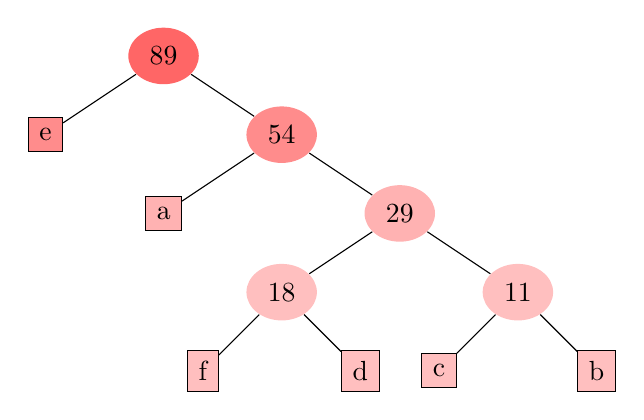
\begin{tikzpicture}
[level distance=10mm,
every node/.style={fill=red!60,ellipse,inner sep=4pt},
level 1/.style={sibling distance=30mm,nodes={fill=red!45}},
level 2/.style={sibling distance=30mm,nodes={fill=red!30}},
level 3/.style={sibling distance=30mm,nodes={fill=red!25}},
level 4/.style={sibling distance=20mm,nodes={fill=red!25}}]
\node {89}
child {node [rectangle,draw]{e}
child [missing]
}
child {node {54}
child {node [rectangle,draw]{a}
}
child {node {29}
child {node {18}
child {node [rectangle,draw]{f}}
child {node [rectangle,draw]{d}}
}
child {node {11}
child {node [rectangle,draw]{c}}
child {node [rectangle,draw]{b}}
}
}
};
\end{tikzpicture}
\end{center}
\end{latin}

\begin{latin}
\rl{کد های ایجاد شده برای حروف }{$ \Rightarrow  a=10 , b=1111 , c=1110 , d=1101 , e=0 , f=1100$}
\end{latin}


\vspace{0.1in}

%Question #14
\question
\vspace{0.5in}

%Question #15
\question
فرض کنید چهار ماتریس زیر را داریم:

\begin{latin}
$A_{20\times2}$ $\times$ $B_{2\times30}$ $\times$ $C_{30\times12}$ $\times$ $D_{12\times8}$
\end{latin}
حداقل تعداد ضرب ها با استفاده از الگوریتم برنامه نویسی پویا کدام است؟
\choice{۳۱۲۰}{۱۲۳۲}{۱۳۲۳}{۲۸۸۰}{b}

\begin{flushright}
\textbf{\color{red}پاسخ :}
\end{flushright}
گزینه ب صحیح می باشد: 
{۱۲۳۲}
\begin{flushright}
\textbf{\color{green}حل :}
\end{flushright}
با بررسی حالت های مختلف:
\begin{latin}
(AB)(CD)(A(B(CD))=30$\times$12$\times$8+2$\times$30$\times$8+20$\times$2$\times$8=3680\\
A((BC)D)=2$\times$30$\times$12+2$\times$12$\times$8+20$\times$2$\times$8=1232\\
(AB)(CD)=20$\times$2$\times$30+30$\times$12$\times$8+20$\times$30$\times$8=8880\\
(A(BC)D)=20$\times$2$\times$30+20$\times$30$\times$12+20$\times$12$\times$8=10320
\end{latin}
ملاحظه می شود گزینه ب برای ضرب این چهار ماتریس صحیح است. 

\vspace{0.1in}

%Question #16
\question 
\vspace{0.5in}

%Question #17
\question
فرض کنید بخواهیم با سه کلید \lr{$key_1<key_2<key_3 $} با احتمالهای جستجوی \lr{$p_3=0.4,p_2=0.3,p_1=0.3 $}یک درخت جستجوی دودوئی بهینه را ایجاد کنیم. کدام نشان دهنده زمان میانگین جستجو در درخت بهینه است؟

\choice{$1.9$}{$1.7$}{$1.6$}{$1.8$}{c}

\begin{flushright}
\textbf{\color{red}پاسخ :}
\end{flushright}
گزینه ج صحیح می باشد: {$1.6$}
\begin{flushright}
\textbf{\color{green}حل :}
\end{flushright}
بهترین حالت ایجاد درخت دودوئی بهینه بصورت زیر می باشد:
\begin{latin}
\usetikzlibrary {shapes.geometric}
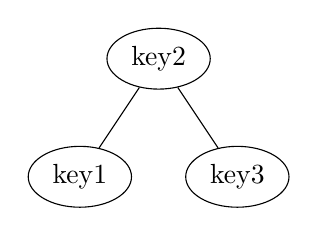
\begin{tikzpicture}[sibling distance=20mm]
\node[ellipse,draw] {key2}
child {node[ellipse,draw] (left node) {key1}}
child {node[ellipse,draw] (right node) {key3}};
\draw[dashed];
\end{tikzpicture}
\end{latin}

\begin{latin}
\begin{center}
\rl{زمان میانگین جستجوی دودوئی }{$= 1 \times 0.4 + 2 \times 0.3 + 2 \times 0.3 = 1.6$}
\end{center}
\end{latin}

\vspace{0.1in}

%Question #18
\question 
\vspace{0.5in}

%Question #19
\question
تعداد درخت های جستجوی دودوئی که می توان با \lr{$5$} کلید متمایز ساخت کدام است؟

\choice{$5$}{$14$}{$42$}{$57$}{c}

\begin{flushright}
\textbf{\color{red}پاسخ :}
\end{flushright}
گزینه ج صحیح می باشد: {$42$}
\begin{flushright}
\textbf{\color{green}حل :}
\end{flushright}
با داشتن \lr{$n$} گره تعداد \lr{$\frac{\dbinom{2n}{n}}{n+1} $} درخت جستجوی دودوئی متفاوت می توان ساخت. حال اگر \lr{$n=5$} باشد داریم: 
\begin{latin}
{$ T(5)=\frac{\dbinom{10}{5}}{5+1}=\frac{10!}{6\times5!\times5!}=\frac{10\times9\times8\times7\times6\times5!}{6\times5!\times5!}=42 $}
\end{latin}

\vspace{0.1in}

%Question #20
\question
\vspace{0.5in}

%Question #21
\question
در حل مسأله یافتن مداره ای همیلتونی درگراف {$G(V,E)$} با استفاده از تکنیک عقبگرد, کدام یک از موارد زیر نشان دهنده غیر امید بخش بودن راس {$i$} ام بر مسیر است ( {$vindex[k]$} اندیس راس بر روی مسیر و {$W[i][j]$} وزن یال از راس {$i$} به راس {$j$} است)؟

\choice
{$i=n-1  \& \& w[vindex[i]][vindex[0]] $}
{$i>0 \& \& (!w[vindex[i-1]][vindex[i]])$}
{$i=n-1 \& \& (!w[videx[i-1]][vindex[0]])$}
{$i>0 \& \& w[vindex[i-1]][vindex[i]]$}
{b} 

\begin{flushright}
\textbf{\color{red}پاسخ :}
\end{flushright}
گزینه ب صحیح می باشد: 
{$i>0 \& \& (!w[vindex[i-1]][vindex[i]])$}

\begin{flushright}
\textbf{\color{green}حل :}
\end{flushright}
یک گراف که توسط یک آرایه دو بعدی W نشان داده شده است که در آن W[i][j] در صورتی True است که بین رأس i ام و j ام یالی وجود داشته باشد و در غیر اینصورت False است.

\vspace{0.5in}

%Question #22
\question
\vspace{0.5in}

%Question #23
\question
کدام گزینه صحیح است؟
\choice
{با روش انشعاب وتحدید زمان اجرا کاهش می یابد.}   
{با روش انشعاب وتحدید حافظه مصرفی کاهش می یابد.}
{با روش انشعاب وتحدید مرتبه زمانی تغییر نمی کند .}
{روش برنامه نویسی پویا, زمان اجرا را کاهش می دهد .}{d}

\begin{flushright}
\textbf{\color{red}پاسخ :}
\end{flushright}
گزینه د صحیح می باشد: 

{روش برنامه نویسی پویا, زمان اجرا را کاهش می دهد .}


\begin{flushright}
\textbf{\color{green}حل :}
\end{flushright}
{روش برنامه نویسی پویا, زمان اجرا را کاهش می دهد .}

\vspace{0.5in}

%Question #24
\question
\vspace{0.1in}

%Question #25
\question
\begin{flushright}
\textbf{\color{red}این برگه شامل ۲۴ سوال تستی می باشد.}
\end{flushright}

\vspace*{\stretch{1}}
\newpage
\end{questions}

%%%%%%%%%%%%%%%%
%%%%%%%%%%%سوالات تشریحی
\begin{center}
\textbf{\color{blue}سوالات تشریحی فرد }
\end{center}

\begin{questions}
%Question #1
\question
رابطه بازگشتی زیر را حل کنید؟


\begin{latin}
\[ T(n) =
  \begin{cases}
   T(n-1)+T(n-2)       & \quad n>2\\
    T(0)=0  & \quad T(1)=1
  \end{cases}
\]
\end{latin}
\begin{flushright}
\textbf{\color{red}پاسخ :}
\end{flushright}
با انتخاب \lr{$T(n)=a_n $} داریم:


\begin{latin}

{$
a_{n} - a_{n-1} - a_{n-4}=0\Rightarrow x^{2}-x-1=0 
\Rightarrow x=\frac {1+\sqrt5}{2} , x=\frac {1-\sqrt5}{2} \Rightarrow\\  
a_n=C_1(1+\frac{\sqrt5}{2})^2 + C_2(1-\frac{\sqrt5}{2})^n \in \theta(1+\frac{\sqrt5}{2})^n
$}
\end{latin}
\vspace*{1in}


%Question #2
\question
\vspace{0.5in}

%Question #3
\question
ماتریس مجاورت گراف جهت دار G که شامل رئوس \lr{$V0 $} تا \lr{$ V4 $} است به صورت زیر داده شده است.الگوریتم دیکسترا را بر روی این گراف برای یافتن کوتاه ترین مسیر از راس منبع \lr{$V0 $} به همه رئوس دیگر کار ببرید؟

\begin{latin}
\[
\begin{array}{lc}
  \verb|| & \begin{bmatrix}
                    \infty & 45 & \infty & 15 & \infty \\
                    \infty & \infty & 20 & 9 & 5 \\
                    \infty & \infty & \infty & \infty & 25 \\
                           5 & 10 & \infty & \infty & 7 \\
                    \infty & 15 & 30 & \infty & \infty
                  \end{bmatrix} \\[15pt]
\end{array}
\]
\end{latin}

\begin{flushright}
\textbf{\color{red}پاسخ :}
\end{flushright}
در مرحله اول کوتاه ترین مسیر از \lr{$V0$} انتخاب می شود که با توجه به گراف مشخص می شود که بهترین گره انتخابی می باشد. بنابراین این مرحله از \lr{$V0$} شروع وبه مستقیما به گره \lr{$V3$} ختم می شود هزینه این مسیر \lr{$15$} خواهد بود و گراف حاصل به صورت زیر خواهد بود:
\begin{latin}
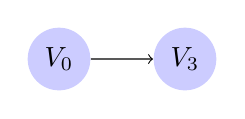
\begin{tikzpicture}[scale=.8,auto=left]
\tikzstyle{every node}=[circle,fill=blue!20]
\node (a) at ( 0,-2) {$V_0$};
\node (b) at ( 2,-2) {$V_3$};
\foreach \from/\to in {a/b}
\draw [->] (\from) -- (\to) {};
\end{tikzpicture}
\end{latin}
\begin{latin}
\begin{center}
\begin{tabular}{ c| c | c | c }

 \rl{گره ها} & S & Dist & P \\ 
\hline
 V\tiny0 & 1 & 0 & V\tiny0 \\  
 V\tiny1 & 0 & 25 &{ V\tiny0}{ V\tiny3}  \\ 
 V\tiny2 & 0 & $\infty$  & V\tiny0 \\ 
 V\tiny3 & 1 & 15 & V\tiny0 \\ 
 V\tiny4 & 0 & 22 & V\tiny0 \\ 
 
\end{tabular}
\end{center}
\end{latin} 
در مرحله دوم مسیری از \lr{$V_0 $} شروع شده و به گره \lr{$V_4 $} ختم می شود بنابراین این مسیر از گره \lr{$V_3 $} نیز می گذرد هزینه گراف حاصل به صورت زیر می باشد:
\begin{latin}
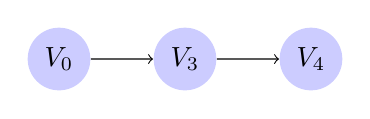
\begin{tikzpicture}[scale=.8,auto=left]
\tikzstyle{every node}=[circle,fill=blue!20]
\node (a) at ( 0,-2) {$V_0$};
\node (b) at ( 2,-2) {$V_3$};
\node (c) at ( 4,-2) {$V_4$};
\foreach \from/\to in {a/b,b/c}
\draw [->] (\from) -- (\to) {};
\end{tikzpicture}
\end{latin}
\begin{latin}
\begin{center}
\begin{tabular}{ c| c | c | c }

 \rl{گره ها} & S & Dist & P \\ 
\hline
 V\tiny0 & 1 & 0 & V\tiny0 \\  
 V\tiny1 & 0 & 25 &{ V\tiny0}{ V\tiny3}  \\ 
 V\tiny2 & 0 & 47 & { V\tiny0}{ V\tiny3}{ V\tiny4} \\ 
 V\tiny3 & 1 & 15 & { V\tiny0}{ V\tiny3} \\ 
 V\tiny4 & 1 & 22 & { V\tiny0}{ V\tiny3}{ V\tiny4} \\ 
\end{tabular}
\end{center}
\end{latin} 
در مرحله سوم مسیری از گره \lr{$V_0 $} شروع شده و به گره \lr{$V_1 $} ختم می شود بنابراین این مسیر از گره \lr{$V_3 $} می گذرد گراف حاصل به صورت زیر می شود:
\begin{latin}
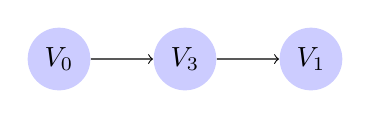
\begin{tikzpicture}[scale=.8,auto=left]
\tikzstyle{every node}=[circle,fill=blue!20]
\node (a) at ( 0,-2) {$V_0$};
\node (b) at ( 2,-2) {$V_3$};
\node (c) at ( 4,-2) {$V_1$};
\foreach \from/\to in {a/b,b/c}
\draw [->] (\from) -- (\to) {};
\end{tikzpicture}
\end{latin}
\begin{latin}
\begin{center}
\begin{tabular}{ c| c | c | c }

 \rl{گره ها} & S & Dist & P \\ 
\hline
 V\tiny0 & 1 & 0 & V\tiny0 \\  
 V\tiny1 & 1 & 25 &{ V\tiny0}{ V\tiny3}{ V\tiny1}  \\ 
 V\tiny2 & 0 & 45 & { V\tiny0}{ V\tiny3}{ V\tiny1} \\ 
 V\tiny3 & 1 & 15 & { V\tiny0}{ V\tiny3} \\ 
 V\tiny4 & 1 & $\infty$ & { V\tiny0} \\ 
\end{tabular}
\end{center}
\end{latin} 
و در مرحله چهارم که مرحله آخر است در این مسیر از گره  \lr{$V_0 $}  شروع شده و به گره  \lr{$V_2 $} ختم می شود بنابراین این مسیر از گره های  \lr{$V_3 $} و  \lr{$V_0 $} می گذرد هزینه این مسیر برابر  {$45 $} است. گراف حاصل به صورت زیر می شود:
\begin{latin}
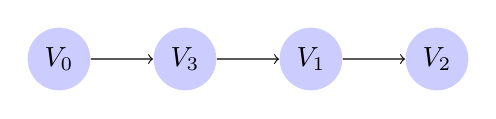
\begin{tikzpicture}[scale=.8,auto=left]
\tikzstyle{every node}=[circle,fill=blue!20]
\node (a) at ( 0,-2) {$V_0$};
\node (b) at ( 2,-2) {$V_3$};
\node (c) at ( 4,-2) {$V_1$};
\node (d) at ( 6,-2) {$V_2$};
\foreach \from/\to in {a/b,b/c,c/d}
\draw [->] (\from) -- (\to) {};
\end{tikzpicture}
\end{latin}

\begin{latin}
\begin{center}
\begin{tabular}{ c| c | c | c }

 \rl{گره ها} & S & Dist & P \\ 
\hline
 V\tiny0 & 1 & 0 & V\tiny0 \\  
 V\tiny1 & 1 & 25 &{ V\tiny0}{ V\tiny3}{ V\tiny1}  \\ 
 V\tiny2 & 0 & 45 & { V\tiny0}{ V\tiny3}{ V\tiny1}{ V\tiny2} \\ 
 V\tiny3 & 1 & 15 & { V\tiny0}{ V\tiny3} \\ 
 V\tiny4 & 1 & 22 & { V\tiny0}{ V\tiny3}{ V\tiny4} \\ 
\end{tabular}
\end{center}
\end{latin}
بنابراین ارزش کل مسیر برابر \lr{$45 $} خواهد بود.
\vspace*{1in}



%Question #4
\question
\vspace{0.5in}

%Question #5
\question
مساله کوله پشتی صفر و یک را برای اجسام \lr{$w1 $}  تا \lr{$w5 $} با ارزش و وزن تعریف شده به صورت زیر و کوله پشتی با وزن \lr{$15 $} کیلو گرم در نظر بگیرید. هدف پر کردن کوله پشتی با اجسام است به نحوی که بیشترین سود حاصل شود. درخت فضای حالت این مساله را با استفاده از روش انشعاب و تحدید رسم نموده و حداکثر سود ممکن را محاسبه نمایید ( اجسام در جدول بر حسب {$p_i/w_i$}مرتب هستند )؟

\begin{latin}
\begin{center}
\begin{tabular}{ l | c | r }
  \rl{جسم} & \rl{ارزش(p)} & \rl{وزن(w)} \\
\hline
  1 & 35\tiny\$ & 7 \\
\hline
  2 & 10\tiny\$ & 2 \\
\hline
  3 & 16\tiny\$ & 4 \\
\hline
 4 & 15\tiny\$ & 5 \\
\hline
  5 & 6\tiny\$ & 6
\end{tabular}
\end{center}
\end{latin}

\begin{flushright}
\textbf{\color{red}پاسخ :}
\end{flushright}
\begin{latin}
\begin{center}
\begin{tabular}{ c| c | c | c }

 \rl{جسم} & \rl{ارزش(p)} & \rl{وزن(w)} & {$\frac{P_i}{W_i}$}\\ 
\hline
 1 & 35\tiny\$ & 7 & 5 \\  
 2 & 10\tiny\$ & 2 & 5  \\ 
 3 & 16\tiny\$ & 4 & 4 \\ 
 4 & 15\tiny\$ & 5 & 3 \\ 
 5 & 6\tiny\$ & 6 & 1 \\ 
\end{tabular}
\end{center}
\end{latin}

\begin{latin}
\begin{center}
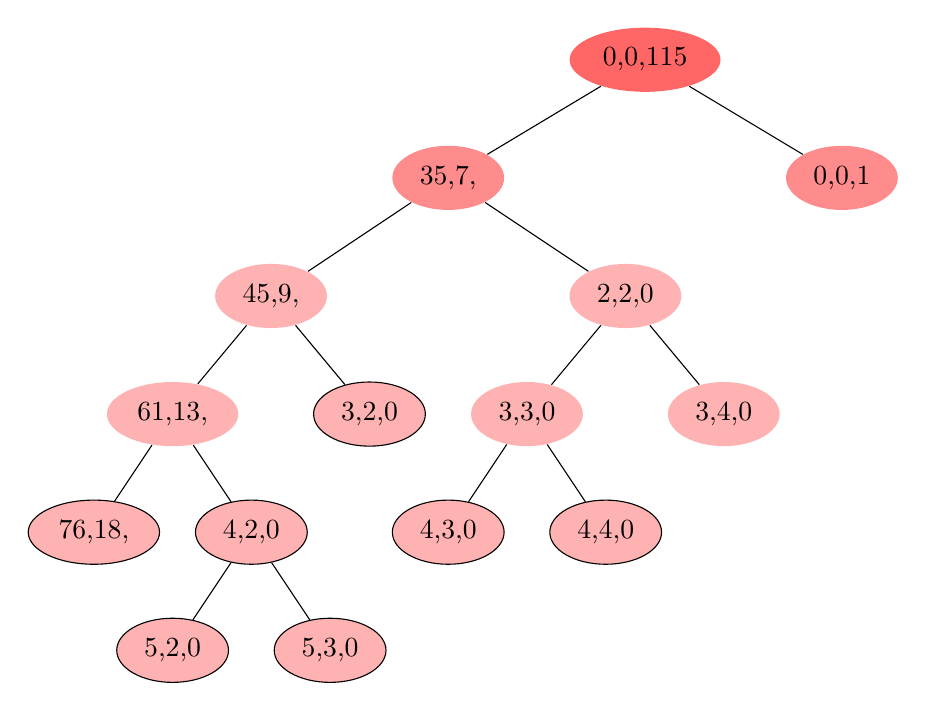
\begin{tikzpicture}
[level distance=15mm,
every node/.style={fill=red!60,ellipse,inner sep=4pt},
level 1/.style={sibling distance=50mm,nodes={fill=red!45}},
level 2/.style={sibling distance=45mm,nodes={fill=red!30}},
level 3/.style={sibling distance=25mm,nodes={fill=red!30}},
level 4/.style={sibling distance=20mm,nodes={fill=red!30}},
level 5/.style={sibling distance=20mm,nodes={fill=red!30}},
level 6/.style={sibling distance=5mm,nodes={fill=red!25}}]
\node {0,0,115}
child {node {35,7,}
child {node {45,9,}
child {node {61,13,}
child {node [ellipse,draw]{76,18,}}
child {node [ellipse,draw]{4,2,0}
child {node [ellipse,draw]{5,2,0}}
child {node [ellipse,draw]{5,3,0}}
}
}
child {node [ellipse,draw]{3,2,0}}
}
child {node {2,2,0}
child {node {3,3,0}
child {node [ellipse,draw]{4,3,0}}
child {node [ellipse,draw]{4,4,0}}
}
child {node {3,4,0}}
}
}
child {node {0,0,1}
};
\end{tikzpicture}
\end{center}
\end{latin}

\vspace*{\stretch{1}}
\newpage

\end{questions}

%%%%%%%%%%%%%%%%%
%\newpage  %Uncomment to put on new age

\bigskip
\begin{center}
\textbf{\color{blue} پاسخ سوالات تستی فرد }
\end{center}
\bigskip  

\showallanswers % 

\end{document}
